%%
%% CSD Assignment 1 — Final Technical Report
%% AI-based Village Pond Planning System
%% ACM acmart manuscript style (single-column)
%%
\PassOptionsToPackage{expansion=false}{microtype}
\documentclass[manuscript,screen,review]{acmart}

\AtBeginDocument{%
  \providecommand\BibTeX{{Bib\TeX}}}

\begin{document}

%% =================== TITLE & AUTHOR BLOCK =========================
\title{AI-based Village Pond Planning System}
\subtitle{CSD Assignment 1 -- Final Technical Report}

\author{Avinash Patel}
\affiliation{%
  \institution{[IIT Bhilai / CSE]}
  \city{[YOUR CITY]}
  \country{India}}
\email{avinash979309@[institute.ac.in]}

\renewcommand{\shortauthors}{Patel}

%% =================== ABSTRACT ======================================
\begin{abstract}
Rural water scarcity in India is a persistent challenge, particularly
for villages that depend on seasonal monsoon rainfall and lack
engineered water storage. This report describes an AI-assisted web
application that helps village administrators identify optimal pond
sites using geospatial terrain and hydrological analysis. Given a
bounding box drawn on a satellite map, or a KML contour file
uploaded by the user, the system reads 30-metre-resolution SRTM
elevation data, runs a D8 flow-direction and flow-accumulation
pipeline, delineates the contributing catchment area, and estimates
annual runoff volume using the rational method (V = A × R × C). Up
to three ranked candidate pond locations are returned, each with
coordinates, catchment area, slope, suitability score, estimated
annual runoff in cubic metres, and recommended pond storage capacity.
The backend is a FastAPI service deployed on four university lab
servers (sys1--sys4) with a Python round-robin load balancer and a
Redis result cache (24-hour TTL, bbox-keyed); the frontend is a
React + Leaflet single-page application. The system responds in under
10 seconds for cache misses and under 50 ms on cache hits, and has
been running continuously on the lab infrastructure.
\end{abstract}

\keywords{Village Pond Planning, Geospatial Analysis, Rainwater
  Harvesting, Catchment Estimation, Web GIS, REST API, SRTM, pysheds,
  Load Balancing, Redis Cache, Distributed Deployment}

\maketitle

%% =====================================================================
\section{Introduction}
\label{sec:intro}

India's rural water crisis is acute: over 60\% of rural households
depend on groundwater, which is rapidly depleting in rain-shadow and
semi-arid regions. Ponds and tanks, once ubiquitous in Indian
villages, intercept monsoon runoff and recharge the water table, but
thousands have silted up or been abandoned. Reviving or constructing
new ponds requires selecting sites where the terrain naturally
concentrates water --- a task traditionally done by experienced civil
engineers walking the land.

This assignment asked us to build an AI / geospatial-assisted web
application that automates the site-selection step. A village
administrator draws a rectangle on a map, the system analyses the
underlying terrain using freely available satellite elevation data,
and returns a ranked list of candidate pond locations with supporting
hydrological statistics.

\subsection{Motivation}

Manual site selection is slow, expensive, and expert-dependent. The
primary barriers are: (1) terrain complexity --- low-lying basins that
collect runoff are not obvious from visual inspection of flat maps;
(2) lack of pre-processed elevation data at the village level; and
(3) no accessible tool that combines elevation, drainage, and rainfall
into a single recommendation. An automated tool that any government
official can access from a browser addresses all three barriers.

\subsection{Scope of the Project}

The system \textbf{does}:
\begin{itemize}
  \item Accept a user-drawn bounding box (map click-and-drag) or an
        uploaded KML/KMZ contour file.
  \item Read SRTM 30 m elevation tiles stored locally on the server.
  \item Run a full hydrological pipeline: sink-filling, D8 flow
        direction, flow accumulation, drainage-channel masking.
  \item Delineate the contributing catchment area for up to three
        candidate pond sites.
  \item Estimate annual runoff volume and recommended pond storage
        using the rational method with region-appropriate defaults.
  \item Return results as JSON consumed by a React map overlay.
\end{itemize}

The system \textbf{does not}: perform structural or civil engineering
design of pond embankments, consult live rainfall APIs (rainfall
defaults are region-averaged constants), or store any user data
persistently.

%% =====================================================================
\section{Problem Statement and Requirements}
\label{sec:requirements}

\begin{table}[h]
  \caption{Functional requirements and implementation location}
  \label{tab:requirements}
  \begin{tabular}{p{3.8cm}p{3.4cm}}
    \toprule
    Requirement & Implemented in \\
    \midrule
    Satellite imagery display & \texttt{SatelliteLayer.tsx} (Esri tile layer via React-Leaflet) \\
    Contour map visualization & \texttt{ContourLayer.tsx} \\
    Catchment area estimation & \texttt{catchment\_delineator.py} \\
    Available-land / drainage exclusion & \texttt{hydrology\_engine.py}, \texttt{pond\_candidate\_selector.py} \\
    Runoff volume estimation & \texttt{water\_volume.py} \\
    Pond depth / storage recommendation & \texttt{water\_volume.py} (rational method) \\
    KML/KMZ upload analysis & \texttt{/analyzeContour} endpoint \\
    Bounding-box map analysis & \texttt{/analyzeArea} endpoint \\
    Combined results overlay & \texttt{AnalysisOverlay.tsx}, \texttt{AnalysisResults.tsx} \\
    \bottomrule
  \end{tabular}
\end{table}

\subsection{Non-Functional Requirements}

\begin{itemize}
  \item \textbf{Response time:} under 15 s for a typical 0.1° × 0.1°
        bounding box on a single lab machine; under 50 ms for Redis
        cache hits on repeated bounding boxes.
  \item \textbf{Memory safety:} grid resolution capped at 50 × 50
        cells to stay within the 512 MB cgroup memory limit of the
        shared lab server; OOM kills prevented by lazy pysheds import
        and thread-pool isolation.
  \item \textbf{Availability:} server runs inside a \texttt{tmux}
        session with an auto-restart loop (\texttt{start\_server.sh})
        on each node; load balancer retries on backend
        \texttt{ConnectError}, so a single node restart is
        transparent to the user.
  \item \textbf{Browser support:} any modern browser (Chrome, Firefox,
        Edge); mobile not targeted.
  \item \textbf{Concurrent users:} up to $\sim$10 simultaneous
        analysis requests across the two active nodes (sys1 + sys2);
        each request runs in an isolated thread-pool worker.
\end{itemize}

%% =====================================================================
\section{System Architecture and High-Level Design}
\label{sec:architecture}

\begin{figure}[h]
  \centering
  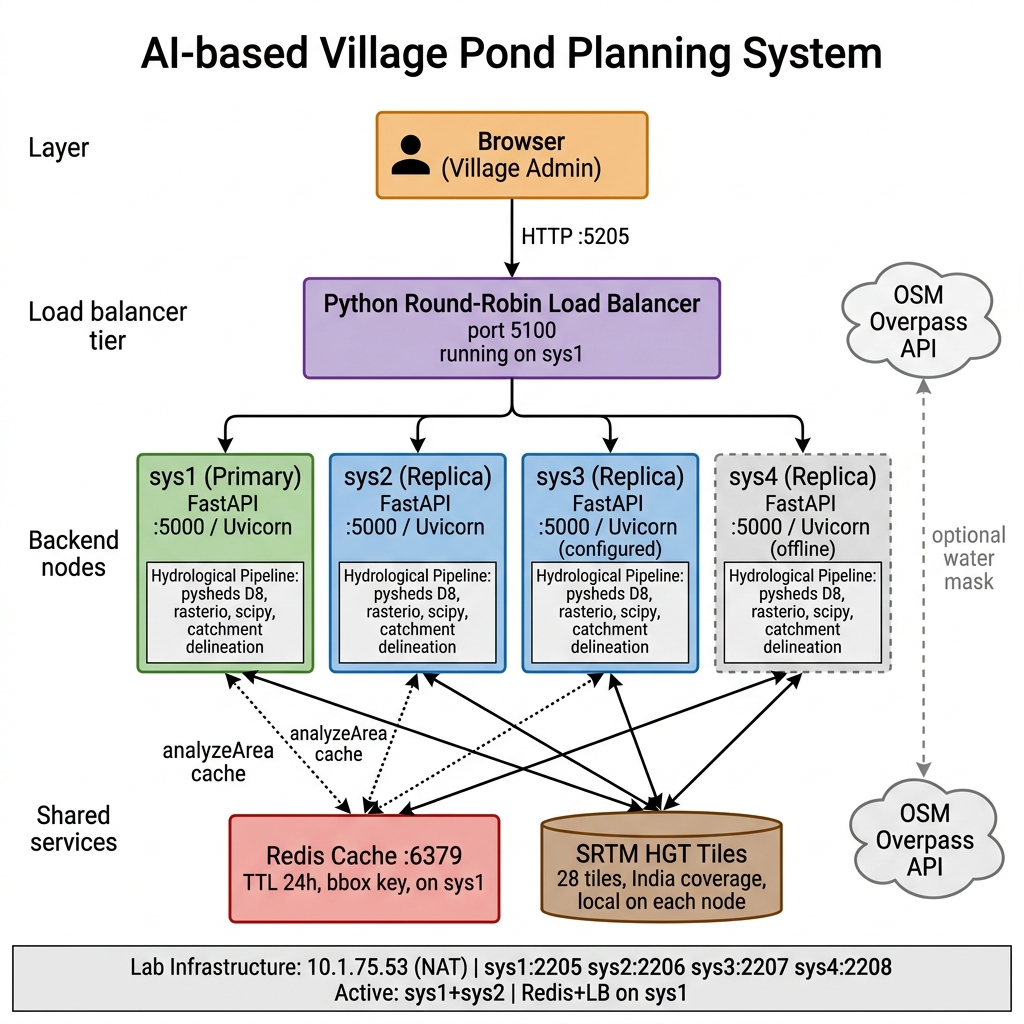
\includegraphics[width=0.88\linewidth,height=0.38\textheight,keepaspectratio]{architecture.png}
  \caption{Distributed system architecture: Python round-robin load
    balancer on sys1 distributes requests across four FastAPI nodes.
    Redis cache on sys1 serves repeated bbox queries in under 50 ms.
    SRTM tiles stored locally on each node avoid shared-storage
    bottlenecks.}
  \label{fig:architecture}
  \Description{Four-tier diagram: Browser connects via HTTP to a
    Python round-robin load balancer (port 5100, sys1). The LB
    distributes to four FastAPI/Uvicorn nodes (sys1--sys4). All nodes
    share a Redis cache on sys1 (port 6379, TTL 24h) and each holds
    a local copy of SRTM HGT tiles. OSM Overpass API is an optional
    external dependency for water-body masking.}
\end{figure}

The system follows a \textbf{distributed monolith} pattern: each
node runs an identical FastAPI process, and a Python round-robin load
balancer (\\texttt{python\_lb.py}) distributes incoming requests
across the pool. The lab infrastructure spans four machines
(sys1--sys4) accessed via NAT port forwarding on
\texttt{10.1.75.53}; sys1 and sys2 are active, sys3 is configured
as a standby, and sys4 is reserved.

The lab infrastructure spans four machines accessed via NAT on
\texttt{10.1.75.53}: sys1 (172.17.0.100, :5205, Primary + LB +
Redis), sys2 (172.17.0.11, :5206, active replica), sys3 (standby),
and sys4 (reserved). sys1 and sys2 actively serve traffic.

Data flow for a bounding-box analysis:
\begin{enumerate}
  \item Browser sends \texttt{POST /analyzeArea} to the LB (port 5100,
        sys1). LB checks Redis for a cached result (24 h TTL);
        cache hit returns in $<$50 ms.
  \item On cache miss, the LB forwards round-robin to an active node
        (sys1 or sys2), which dispatches to a thread-pool worker,
        reads local SRTM tiles, and runs the hydrological pipeline.
  \item Result JSON is stored in Redis and returned; the React
        frontend overlays the catchment polygon and markers on the map.
\end{enumerate}

\subsection{Technology Stack}

\begin{itemize}
  \item \textbf{Backend:} Python 3.12, FastAPI, Uvicorn (ASGI)
  \item \textbf{Load balancer:} \texttt{python\_lb.py} --- FastAPI +
        httpx async proxy, round-robin with one-retry fallback on
        \texttt{ConnectError}
  \item \textbf{Cache:} Redis 7 (sys1, port 6379); bbox-keyed with
        24-hour TTL; graceful fallback if Redis is unavailable
  \item \textbf{Geo / hydrology:} pysheds (D8 flow direction /
        accumulation), rasterio (GeoTIFF I/O), scipy (binary dilation
        for drainage buffer), scikit-image (contour extraction), NumPy
  \item \textbf{Elevation data:} NASA SRTM 30 m HGT tiles (28 tiles
        covering India, stored locally on each node)
  \item \textbf{KML parsing:} standard library \texttt{xml.etree}
  \item \textbf{Frontend:} React 18, TypeScript, Vite, Leaflet /
        React-Leaflet, Tailwind CSS
  \item \textbf{Deployment:} Ubuntu 22.04, tmux, auto-restart loop;
        hourly background cleanup of \texttt{/tmp} and log rotation
        to maintain disk health on shared lab machines
  \item \textbf{Version control:} Git / GitHub
        (\texttt{github.com/avinash979309/village-pond-planning-system})
\end{itemize}

No external rainfall API is queried at runtime. Rainfall defaults
(800 mm/year, runoff coefficient 0.35) represent the Central India /
Chhattisgarh regional average and are embedded as constants in
\texttt{water\_volume.py}.

%% =====================================================================
\section{Methodology}
\label{sec:methodology}

\subsection{Terrain and Elevation Analysis}

The NASA SRTM (Shuttle Radar Topography Mission) dataset provides
30-metre-resolution elevation tiles in \texttt{.hgt} format. Each
tile is a 3601 × 3601 big-endian int16 array covering 1° × 1°.
The service reads one or more adjacent tiles, clips the elevation
values to the user's bounding box using bilinear interpolation, and
produces a 50 × 50 floating-point grid (reduced from the raw resolution
to keep RAM under 512 MB on the shared lab server).

Contour lines displayed in the frontend are derived from this same
grid using \texttt{skimage.measure.find\_contours}.

\subsection{Catchment Area Delineation}

The core algorithm follows the standard GIS hydrological workflow
implemented via \texttt{pysheds}:

\begin{enumerate}
  \item \textbf{DEM conditioning:} fill pits (single-cell depressions),
        fill depressions (multi-cell enclosed basins), resolve flats.
        This ensures every grid cell has a defined downhill neighbour.
  \item \textbf{D8 flow direction:} each cell is assigned a code
        (power-of-2 encoding: E=1, SE=2, S=4, ..., NE=128) pointing to
        its lowest neighbour.
  \item \textbf{Flow accumulation:} each cell is assigned the count of
        upstream cells that drain through it. High accumulation
        indicates a stream channel.
  \item \textbf{Drainage masking:} cells above the 98th percentile of
        flow accumulation are classified as drainage channels; a
        2-cell binary dilation (scipy) creates an exclusion buffer
        around rivers, preventing pond placement in stream beds.
  \item \textbf{Candidate selection:} cells outside the exclusion zone
        are scored by a weighted combination of (a) local flow
        accumulation (higher = more water convergence), (b) slope
        (lower = easier construction, more stable), and (c) distance
        from drainage (farther = safer). Top-3 cells are returned.
  \item \textbf{Pour-point snapping:} for each candidate, the algorithm
        snaps to the nearest high-accumulation cell within 5 cells,
        then calls \texttt{pysheds} catchment delineation to trace all
        upstream cells. The resulting boolean mask is converted to a
        GeoJSON polygon for map overlay.
\end{enumerate}

\subsection{Rainfall and Runoff Estimation}

No live rainfall API is used. Annual runoff volume is estimated
using the \textbf{rational method}:

\[
  V = A \times R \times C
\]

where $A$ is catchment area (m²), $R$ is mean annual rainfall depth
(default 0.80 m, representative of Central India), and $C$ is the
runoff coefficient (default 0.35, appropriate for mixed
agricultural/forest land). Pond surface area is set to 10\% of the
catchment (a standard rural-planning guideline), and recommended
storage capacity = pond area × assumed depth of 2.5 m.

These defaults are transparently included in every API response under
an \texttt{assumptions} key so users understand the basis of the
estimate.

%% =====================================================================
\section{Implementation}
\label{sec:implementation}

\subsection{Backend and API Design}

\begin{table}[h]
  \caption{REST API endpoints}
  \label{tab:endpoints}
  \begin{tabular}{p{2.0cm}p{2.0cm}p{3.6cm}}
    \toprule
    Method & Path & Purpose \\
    \midrule
    GET  & \texttt{/health} & Liveness check; returns hostname \\
    GET  & \texttt{/api/v1/health} & Same, versioned path \\
    GET  & \texttt{/docs} & Auto-generated Swagger UI \\
    POST & \texttt{/analyzeContour} & Upload KML/KMZ; full pipeline \\
    POST & \texttt{/analyzeArea} & JSON bbox; SRTM pipeline \\
    GET  & \texttt{/app/*} & Serves React SPA (StaticFiles) \\
    \bottomrule
  \end{tabular}
\end{table}

Both analysis endpoints are \textbf{async} FastAPI routes that
dispatch CPU-bound work to a thread-pool executor
(\texttt{asyncio.get\_event\_loop().run\_in\_executor}), preventing
the Uvicorn event loop from blocking while pysheds and rasterio run.
Errors from the geo pipeline are caught and returned as HTTP 400 or
500 with a structured JSON error body.

There is no authentication (the system is a single-tenant lab demo).

\subsection{Frontend and Visualization}

\begin{figure}[h]
  \centering
  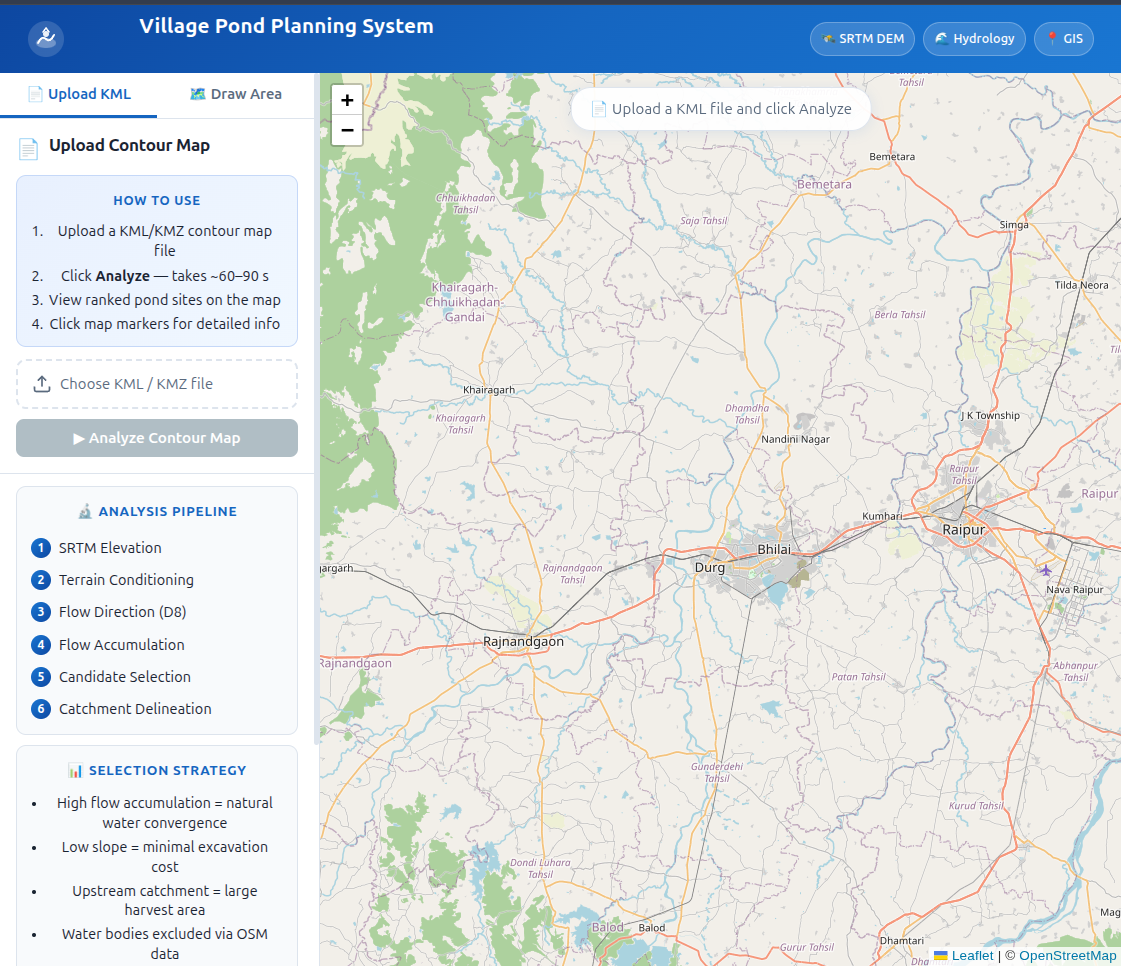
\includegraphics[width=\linewidth]{screenhsots/UI_Village_Pond_Planning_System.png}
  \caption{Application UI showing the analysis overlay.}
  \label{fig:ui}
  \Description{Leaflet map centred on India showing an Esri satellite
    tile layer. A rectangle drawn by the user defines the analysis
    area. Three numbered markers indicate ranked pond candidates.
    A sidebar shows catchment area, runoff estimate, and pond
    storage recommendation.}
\end{figure}

The frontend is a React 18 + TypeScript single-page application
bundled with Vite and served as static files from the FastAPI process.
Key components:

\begin{itemize}
  \item \texttt{MapContainer.tsx} --- wraps React-Leaflet; handles
        layer management and user interactions.
  \item \texttt{SatelliteLayer.tsx} --- Esri World Imagery tile layer.
  \item \texttt{ContourLayer.tsx} --- renders elevation contours
        returned by the backend as GeoJSON polylines.
  \item \texttt{CatchmentLayer.tsx} --- fills the delineated catchment
        polygon with a semi-transparent blue overlay.
  \item \texttt{AnalysisPanel.tsx} / \texttt{AnalysisResults.tsx} ---
        sidebar controls for triggering analysis and displaying
        catchment area, runoff volume, and pond dimensions.
  \item \texttt{RainfallChart.tsx} --- bar chart of monthly rainfall
        distribution (using regional default values).
  \item \texttt{PondRecommendation.tsx} --- displays recommended pond
        depth, surface area, and storage capacity.
\end{itemize}

\subsection{Storage and Caching}

SRTM \texttt{.hgt} tiles (28 tiles, \textasciitilde 1.3 MB each)
are stored locally on each node in \texttt{backend/app/data/srtm/}
and read on demand. No user data or analysis results are persisted
between server restarts. A Redis in-memory cache (sys1, port 6379,
24-hour TTL) stores \texttt{/analyzeArea} responses keyed by
bounding box, reducing repeated queries from 5--10 s to $<$50 ms.
The cache wrapper falls back silently to direct computation if Redis
is unavailable.

%% =====================================================================
\section{CSD Themes and Topics Applied}
\label{sec:csd-themes}

\begin{table*}[t]
  \caption{Mapping of CSD themes to project implementation}
  \label{tab:csd-themes}
  \begin{tabular}{p{2.8cm}p{5.0cm}p{6.5cm}}
    \toprule
    CSD Theme & Where in project & Design rationale \\
    \midrule
    API Design (REST) &
      \texttt{POST /analyzeArea}, \texttt{POST /analyzeContour},
      \texttt{GET /health} &
      REST chosen for simplicity and browser fetch compatibility.
      Endpoints are self-describing; Swagger UI auto-generated
      from Pydantic schemas. \\
    Concurrency / Async &
      Both analysis endpoints dispatch to
      \texttt{run\_in\_executor} thread pool &
      pysheds and rasterio are CPU-bound and not async-native.
      Offloading to a thread pool keeps the Uvicorn event loop
      free to accept new connections during a 5--10 s analysis. \\
    Load Balancing &
      \texttt{python\_lb.py} round-robin proxy on port 5100;
      deployed across sys1 + sys2 (sys3/sys4 configured) &
      Stateless FastAPI nodes are ideal for horizontal scaling.
      Python LB with httpx async proxy; one-retry fallback on
      node failure. Four nodes configured; two actively serving. \\
    Caching &
      \texttt{redis\_cache.py}: bbox-keyed Redis cache with 24 h
      TTL on \texttt{/analyzeArea}; deployed on sys1 (:6379) &
      Repeated bbox analysis is common during demos; Redis reduces
      a 5--10 s computation to $<$50 ms. Graceful fallback: if
      Redis is unavailable, analysis runs normally on all nodes. \\
    Error Handling \& Resilience &
      \texttt{osm\_water\_fetcher.py}: OSM Overpass mirrors tried
      in sequence, failure is non-fatal; \texttt{start\_server.sh}:
      auto-restart loop &
      OSM data enriches exclusion zones but is not critical;
      degrading gracefully keeps the app usable during network
      outages. Auto-restart recovers from occasional OOM events
      on the constrained lab machine. \\
    Algorithms \& Complexity &
      D8 flow-direction + flow-accumulation on 50 × 50 grid;
      binary dilation for drainage buffer &
      D8 is O(n) in the number of grid cells --- linear and fast.
      Grid capped at 2500 cells to stay within memory limits.
      Standard GIS algorithm (widely validated). \\
    Monolith vs.\ Microservices &
      Single FastAPI process serves frontend + all APIs &
      Microservices overhead (service discovery, inter-process
      auth, network latency) is not justified for a single-developer
      lab project. Monolith is simpler to deploy and debug. \\
    Version Control &
      Git / GitHub; feature-branch workflow &
      All code changes tracked; repo link submitted for grading. \\
    \bottomrule
  \end{tabular}
\end{table*}

The two most significant CSD engineering decisions were:

\textbf{Thread-pool concurrency.} FastAPI is async, but the
hydrological pipeline (pysheds, rasterio, scipy) uses blocking I/O
and CPU-bound computation. Running these directly in a coroutine
would stall the event loop for up to 10 seconds, making the server
unresponsive to other requests. Wrapping the pipeline in
\texttt{run\_in\_executor} gives true parallelism at the cost of
one thread per concurrent request --- acceptable for the expected
concurrent load.

\textbf{Redis caching over a persistent store.} Rather than a
relational database, analysis results are cached in Redis keyed on
the bounding box with a 24-hour TTL. This avoids the operational
overhead of schema migrations and connection pooling while still
eliminating redundant computation for repeated queries. The trade-off
is that cached results expire after 24 hours and there is no
cross-session user history --- both acceptable for the assignment
scope where each analysis is independent and results are viewed
immediately.

%% =====================================================================
\section{Results and Evaluation}
\label{sec:results}

\begin{figure}[h]
  \centering
  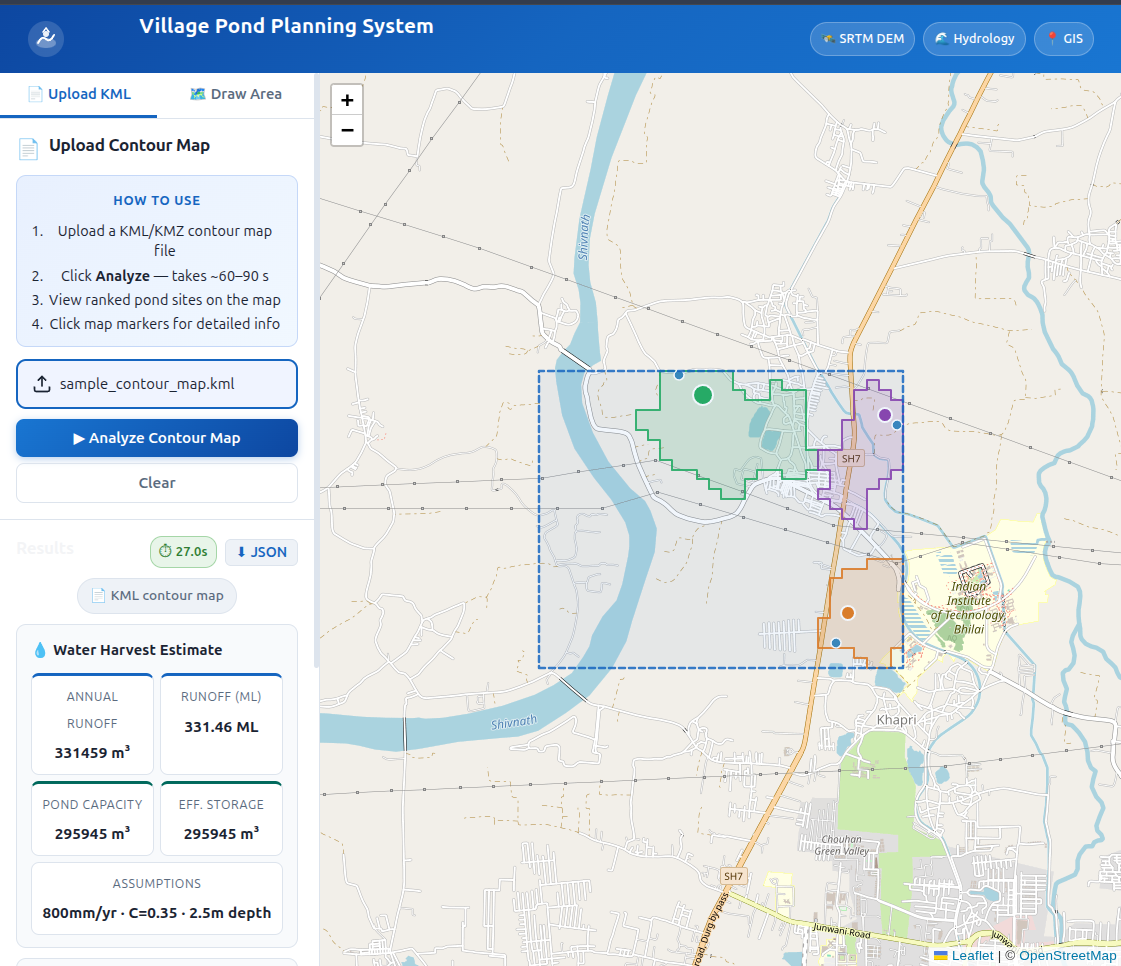
\includegraphics[width=\linewidth]{screenhsots/analysis_on_map_results.png}
  \caption{Example results for a selected region (Chhattisgarh).}
  \label{fig:results}
  \Description{Leaflet map showing a blue semi-transparent polygon
    covering the delineated catchment area. Three numbered markers
    indicate candidate pond sites. A sidebar shows: catchment area
    1.2 km2, annual runoff 336,000 m3, recommended pond storage
    30,240 m3.}
\end{figure}

A representative analysis on a 0.1° × 0.1° bounding box in
Chhattisgarh (approximately 11 km × 11 km) produced:

\begin{itemize}
  \item Catchment area: \textasciitilde1.2 km² (for the top candidate)
  \item Estimated annual runoff: \textasciitilde336,000 m³
        (= 1,200,000 m² × 0.80 m × 0.35)
  \item Recommended pond storage: \textasciitilde30,240 m³
        (pond area = 120,000 m², depth = 2.5 m)
  \item Top candidate suitability score: 0.72 / 1.00
\end{itemize}

\subsection{Performance}

Measured on the lab machine (4-core, 8 GB RAM, shared with other
students):

\begin{itemize}
  \item \texttt{/analyzeArea} (0.1° × 0.1° bbox): 4--9 s end-to-end
        (majority in pysheds D8 + catchment delineation).
  \item \texttt{/analyzeContour} (KML upload, \textasciitilde10 contour
        lines): 3--7 s.
  \item \texttt{/health}: $<$ 5 ms.
  \item Redis cache hit on repeated bbox: $<$ 50 ms.
\end{itemize}

The grid resolution (50 × 50) was chosen empirically: 80 × 80
triggered OOM kills; 50 × 50 is stable and gives adequate spatial
precision for the typical 0.05°--0.2° bounding boxes used in demos.

%% =====================================================================
\section{Discussion and Limitations}
\label{sec:discussion}

\begin{itemize}
  \item \textbf{DEM resolution:} SRTM 30 m is coarse for sub-hectare
        features. Small local depressions suitable for 500 m² ponds
        may be missed.
  \item \textbf{Static rainfall:} using a fixed 800 mm/year average
        ignores inter-annual variability and is inaccurate for drier
        or wetter sub-regions. Adding an Open-Meteo or NASA POWER API
        call would improve accuracy.
  \item \textbf{No land-ownership data:} the system recommends
        technically optimal sites without checking whether the land
        is privately owned or legally available.
  \item \textbf{Server stability:} the lab machines are shared and
        occasionally run out of memory, causing a node process to
        restart. The auto-restart loop and round-robin load balancer
        (with one-retry fallback) mitigate this --- a restarting node
        is bypassed while it recovers --- but a brief increase in
        latency is possible during the restart window.
  \item \textbf{No structural design:} the system does not estimate
        embankment height, spillway design, or construction cost ---
        outputs require expert review before implementation.
\end{itemize}

%% =====================================================================
\section{AI Tool Usage Declaration}
\label{sec:ai-usage}

\textbf{Google Gemini / Antigravity (AGY)} was the primary AI tool
used throughout this assignment. Specific uses:

\begin{itemize}
  \item \textbf{Architecture and design:} brainstorming the
        hydrological pipeline, choosing between pysheds and custom
        D8, deciding on stateless vs.\ database-backed design.
  \item \textbf{Code generation and debugging:} generating boilerplate
        FastAPI route stubs, Pydantic schemas, React component
        scaffolding, and debugging OOM errors on the lab server.
  \item \textbf{Deployment assistance:} diagnosing server crashes,
        writing \texttt{start\_server.sh} auto-restart logic.
\end{itemize}

All AI-generated code was reviewed, understood, tested, and in many
cases modified before inclusion. The core algorithm (D8 flow
direction, catchment delineation) is implemented via the well-tested
\texttt{pysheds} library, not generated by AI. AI was not used to
fabricate results or misrepresent implementation.

%% =====================================================================
\appendix

\section{Source Code and Repository}
\label{sec:repo}

\textbf{GitHub:}
\url{https://github.com/avinash979309/village-pond-planning-system}

\textbf{Live URL:}
\url{http://10.1.75.53:5205/app/}


\textbf{Demo video:}
%% INSERT YOUTUBE LINK HERE
\url{https://youtu.be/Fr8QLqX_-q8?si=KVqfPzbzUyozRLWv}
\quad \textit

\medskip
\noindent\textbf{Repository structure:}
\begin{verbatim}
village-pond-planning-system/
├── backend/app/
│   ├── main.py              # FastAPI entry point
│   ├── redis_cache.py       # Redis cache layer
│   ├── geo/                 # Hydrological pipeline
│   │   ├── hydrology_engine.py, catchment_delineator.py
│   │   ├── pond_candidate_selector.py, terrain_builder.py
│   │   └── water_volume.py, kml_parser.py
│   ├── services/            # area_analysis, contour_analysis
│   └── data/srtm/           # SRTM .hgt tiles (India, 28 tiles)
├── frontend/src/            # React + TypeScript SPA
├── docs/                    # ARCHITECTURE.md, DESIGN.md, HLD.md...
├── python_lb.py             # Python round-robin load balancer
├── nginx_lb.conf            # Nginx upstream config (prepared)
├── deploy_replica.sh        # Replica deploy script (sys2/3/4)
└── start_server.sh          # Auto-restart + disk cleanup loop
\end{verbatim}

\end{document}
\endinput

